\documentclass[border=5pt]{standalone}
\usepackage{tikz}
\usetikzlibrary{angles,quotes}

\newcommand\Base[1][0]{
\begin{scope}[xshift=#1]
\clip
  (-0.5,5.5) rectangle (5.5,-0.5);
  \draw[->]
  (-0.5,0) -- (5,0) node[right] {$u$};
\draw[->]
  (0,-0.5) -- (0,5) node[above] {$v$};
\coordinate (O) at (0,0);
\coordinate (aux1) at (40:4);
\coordinate (aux2) at (aux1|-0,0);
\coordinate (aux3) at (4,{4*tan(40)});
\draw
  (O) -- (aux3) -- (aux3|-0,0)
  (aux1) -- (aux2);
\draw[thick,red!70!black]
  (O) circle (4);
\pic[draw,"$\alpha$",angle radius=30pt,angle eccentricity=1.2] {angle = aux2--O--aux1};
\end{scope}
}

\begin{document}

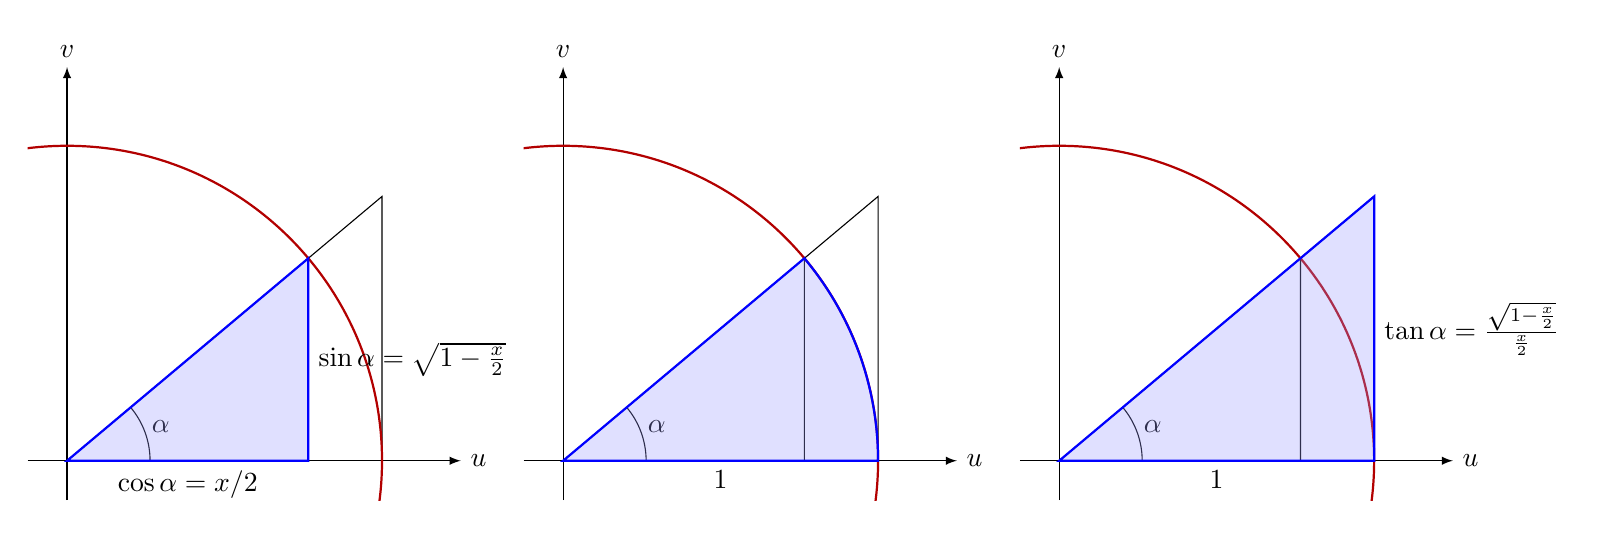
\begin{tikzpicture}[>=latex]
\Base
\filldraw[thick,draw=blue,fill=blue!40,fill opacity=0.3,text opacity=1]
  (O) -- (aux1) -- node[right] {$\sin \alpha=\sqrt{1-\frac{x}{2}}$} (aux2)  -- node[below] {$\cos \alpha=x/2$} cycle;

\Base[6.3cm]
\filldraw[thick,draw=blue,fill=blue!40,fill opacity=0.3,text opacity=1]
  (O) -- (aux1) arc (40:0:4) -- node[below] {$1$} cycle;

\Base[12.6cm]
\filldraw[thick,draw=blue,fill=blue!40,fill opacity=0.3,text opacity=1]
  (O) -- (aux3) -- node[right] {$\tan \alpha=\frac{\sqrt{1-\frac{x}{2}}}{\frac{x}{2}}$} (aux3|-0,0)  -- node[below] {$1$} cycle;

\end{tikzpicture}

\end{document}
